\documentclass[
12pt, % Main document font size
a4paper
%, % Paper type, use 'letterpaper' for US Letter paper
%oneside, % One page layout (no page indentation)
%twoside, % Two page layout (page indentation for binding and different headers)
%headinclude,footinclude, % Extra spacing for the header and footer
%BCOR5mm, % Binding correction
]{report}

\usepackage[font=small,labelfont=bf,justification=raggedright,format=hang,singlelinecheck=off,textfont=it]{caption}
%\usepackage{subcaption}
\usepackage{indentfirst}
\usepackage{longtable}
\usepackage{tabu}
\usepackage{titlepic}
\usepackage{geometry}
\geometry{margin=1in,top=1.5in,bottom=1.5in}
\usepackage{mathtools}
\usepackage{polski}
\usepackage[utf8]{inputenc}
\usepackage{booktabs}
\usepackage[T1]{fontenc}
\usepackage{lmodern}
\usepackage{fancyhdr}
\pagestyle{fancy}
\pagestyle{headings}
\usepackage{float}
\usepackage{graphicx}
\usepackage{listings}
\usepackage{enumitem}
\usepackage{titlesec}
\usepackage{pdfpages}
\usepackage{wallpaper}
\usepackage{cleveref}
\usepackage{afterpage}

\usepackage{hyperref}
\hypersetup{
    colorlinks,
    citecolor=black,
    filecolor=black,
    linkcolor=black,
    urlcolor=black
}

\newcommand\blankpage{%
    \null
	\ClearWallPaper
    \thispagestyle{empty}%
    \addtocounter{page}{-1}%
    \newpage
	\ULCornerWallPaper{1}{head}}

%\captionsetup{}

%\usepackage{showframe}


\newcounter{magicrownumbers}
\newcommand\rownumber{\stepcounter{magicrownumbers}\arabic{magicrownumbers}}

%variables
\newcommand{\shopname}{SHOP NAME}
\newcommand{\companyname}{COMPANY NAME}
\newcommand{\regon}{REGON}
\newcommand{\nip}{NIP}
\newcommand{\httpaddr}{SITE ADDRESS}
\newcommand{\address}{ADDRESS}
\newcommand{\mail}{MAIL ADDRESS}
\newcommand{\phone}{PHONE NUMBER}
\newcommand{\currency}{CURRENCY}

\setlistdepth{9}
\graphicspath{ {images/} }

\title{Biznes plan sklep-meblowy.org}
\author{Kamila Klonowska <kamila.klon@sklep-meblowy.org>}
\titlepic{
\includegraphics[width=128px]{logo.png}}

%definitions
\newif\ifpersonal
\personaltrue % comment out to hide answers

%styling
\titlespacing*{\subparagraph}{1em}{0pt}{0pt}
\titleformat{\subparagraph}[runin]
{\normalfont\normalsize}{\thesubparagraph}{1em}{}

\ULCornerWallPaper{1}{head}
%\LLCornerWallPaper{1}{foot}

\begin{document}			


	%strona tytulowa
	\begin{titlepage}
	\clearpage\maketitle
	\thispagestyle{empty}
\end{titlepage}


	\afterpage{\blankpage}
	
	%spis tresci
	% Set the depth of the table of contents to show sections and subsections only
%\setcounter{tocdepth}{2} 
\newpage 
\tableofcontents % Print the table of contents
\newpage

	
	\chapter{Uzasadnienie cen}
	\section{Analiza rynku}
		\par Na potrzeby polityki cenowej przeprowadzona została wstępna analiza rynku obejmująca badanie statystyczne najpopularniejszych portali aukcyjnych w Polsce i Kanadzie. Przebadane portale to ebay.ca i allegro.pl. Metodyką przeprowadzonej analizy było zestawienie pięciu par podobnych między sobą artykułów, a następnie wyliczenie na tej podstawie średniej arytmetycznej. Na podstawie przeprowadzonej analizy udało się ustalić następujące ceny średnie artykułów z danych grup:
		
		\begin{table}[H]
		\centering
		\begin{tabular}{|l|l|l|}
		\hline
					& Polska [zł] & Kanada [zł]\\ \hline
		Komody 	& 384  & 2613 \\ \hline
		Fotele 	& 1058 & 2943 \\ \hline
		Sofy   	& 3729 & 9611 \\ \hline
		Stoły  	& 1185 & 3366 \\ \hline
		Łóżka  	& 1355 & 6145 \\ \hline
		\end{tabular}
		\caption{Średnia cena grup produktów w Polsce i Kanadzie}
		\label{avg_grp_price_ca_pl}
		\end{table}

		Ponadto dzięki powziętej analizie udało się wyliczyć średnią cenę towarów Polsce jak i w Kanadzie. Średnia cena w Polsce wynosi 1831 zł, a w Kanadzie 5516 zł. Co daje różnicę w cenie średniej w wysokości 3685 zł. Jest potencjalny zarobek w przypadku eksportu. Jednak dla określenia polityki cenowej istotne jest jeszcze określenie średniej ceny transportu towaru od producenta do klienta. Na tę potrzebę przeprowadzono analizę dokładnie tą samą metodologią. Jej wyniki prezentuję tabela poniżej.
		
		\begin{table}[H]
		\centering
		\begin{tabular}{|l|l|l|l|}
		\hline
					& Polska \textless-\textgreater Polska [zł] & Kanada \textless-\textgreater Kanada [zł] & Polska \textless-\textgreater Kanada [zł] \\ \hline
		Komody 	& 69                                 & 414                                & 960                                \\ \hline
		Fotele 	& 51                                 & 408                                & 960                                \\ \hline
		Sofy   	& 480                                & 1225                               & 1606                               \\ \hline
		Stoły  	& 94                                 & 1137                               & 960                                \\ \hline
		Łóżka  	& 321                               	& 1167                               & 1200                               \\ \hline
		\end{tabular}
		\caption{Średnia cena transportu wybranych grup produktów}
		\label{avg_grp_shp_price}
		\end{table}
		
		Dzięki tej analizie ustalono, że średnia cena wysyłki towaru w Polsce wynosi 203zł, cena wysyłki w Kanadzie wynosi 870zł, a przesyłki z Polski do Kanady 1137zł. Na tej podstawie można ustalić średnią kwotę wysyłki produktu z Polski do Kanady, na którą składać się będą wysyłka z Polski do Kanady oraz wysyłka na terenie Kanady. Nie wlicza się w nią natomiast cena transportu w Polsce, ponieważ wybrane firmy spedycyjne dysponują własną flotą na terenie Polski. Na tej podstawie średni koszt wysyłki oszacować można na 2007 zł.
		
		Na podstawie powyższych analiz można sformułować ogólny zarys cen obowiązujących na rynku, polskim średnia cena produktu 1831 zł, a średni koszt transportu 203zł. Natomiast dla rynku kanadyjskiego 5516 zł, średni koszt transportu to 870zł, oraz przedstawić poniższą tabelę zawierającą ceny średnie powiększone o średni koszt transportu.
		
		\begin{table}[H]
		\centering
		\begin{tabular}{|l|l|l|}
		\hline
					& Polska [zł]& Kanada [zł]\\ \hline
		Komody 	& 453  & 3027 \\ \hline
		Fotele 	& 1109 & 3351 \\ \hline
		Sofy   	& 4209 & 10836 \\ \hline
		Stoły  	& 1279 & 4503 \\ \hline
		Łóżka  	& 1676 & 7312 \\ \hline
		\end{tabular}
		\caption{Średnia cena produktu w Polsce i Kanadzie powiększona o średni koszt transportu}
		\label{avg_price_pl_ca}
		\end{table}

		Na podstawie powyższych można ustalić  następującą politykę cen dla Polski i dla Kanady. Korzystając z danych GUS o polskim rynku wewnętrznym można ustalić marżę na 20\%. Co do rynku kanadyjskiego na podstawie powyższych udało się ustalić, że średnia cena produktu produktu w Polsce wraz z transportem do Kanady stanowi ok 55\% ceny towaru w Kanadzie wraz z transportem. Na tej podstawie marżę dla rynku kanadyjskiego można ustalić na poziomie 100\% ceny produktu w Polsce. 
		
		
		
		\begin{figure}[H]
			\centering
			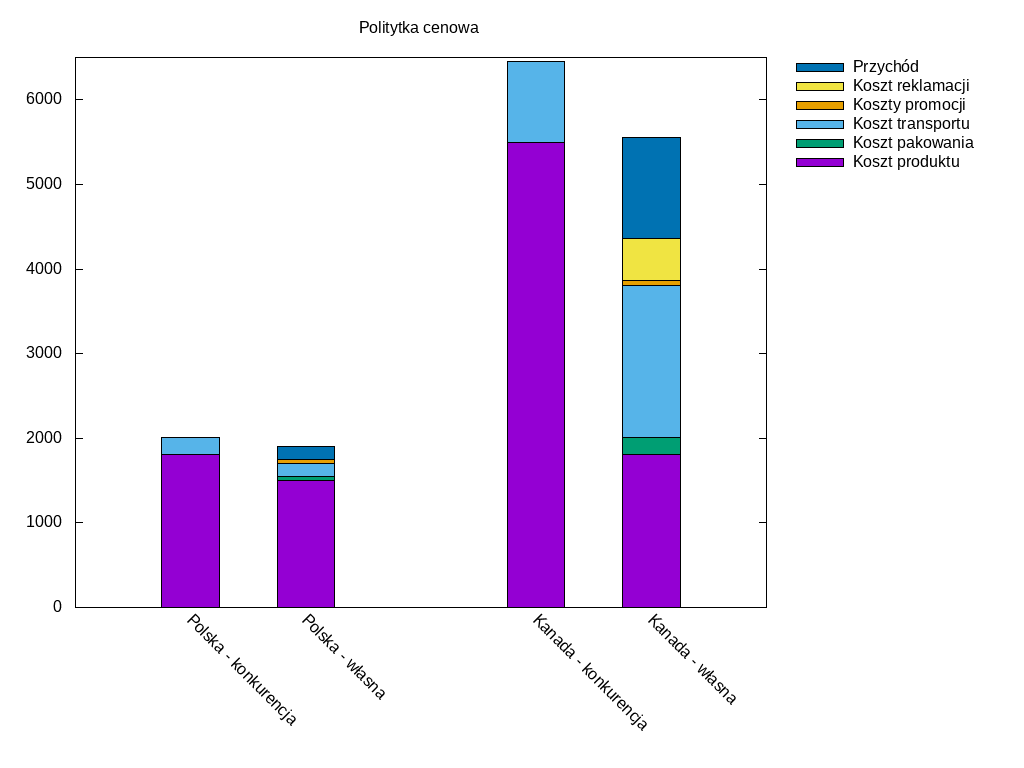
\includegraphics[scale=0.5]{polityka_cen}
			\caption{Polityka cenowa w Polsce i Kanadzie}
			\label{polityka_cen}
		\end{figure}

        
		
		
\end{document}
